\section{Consuntivazione}

\subsection{Milestones:}
\begin{itemize}
    \item Analisi dei requisiti v1.0.0 (Completa al: 50\%)
    \item Requirements and technology baseline (Completa al: 30\%)
\end{itemize}

\subsection{Attività svolte}


\begin{table}[ht]
    \begin{tabularx}{\textwidth}{X l l}
        
        \rowcolor{gray!30} \textbf{Attività} & \textbf{Stato} & \textbf{Ruolo}\\
        
        \hline
        creazione di un ambiente \textit{github pages} & completato & Amministratore\\
    \end{tabularx}
    \caption{Lista delle attività svolte durante lo sprint}
\end{table}


\begin{table}[ht]
    \begin{tabularx}{\linewidth}{X|rrrrrrr}
    \rowcolor{gray!30}& Re & Amm & An & Pro & Prog & Ver & tot \\
    \hline
    Bonavigo Michele                        & 0 & 0 & 0 & 0 & 0 & 0  & 0 \\
    \rowcolor{gray!10}Casarotto Mattia      & 0 & 0 & 0 & 0 & 0 & 0  & 0 \\
    Massarenti Alessandro                   & 0 & 0 & 0 & 0 & 0 & 0  & 1 \\
    \rowcolor{gray!10}Peron Samuel          & 2,5 & 0 & 0 & 0 & 0 & 0 & 0\\
    Pierobon Luca                           & 0 & 3 & 0 & 0 & 0 & 0 & 0\\
    \rowcolor{gray!10}Romano Davide         & 0 & 0 & 0 & 0 & 0 & 0 & 0\\
    Zarantonello Giorgio                    & 0 & 0 & 0 & 0 & 0 & 0 & 0 \\
    \hline                                  & 2,5 & 3 & 0 & 0 & 0 & 1 & 
    \end{tabularx}
    \caption{\label{ruoli-persone}Spartizione dei ruoli e ore svolte durante lo sprint}
\end{table}

\begin{center}
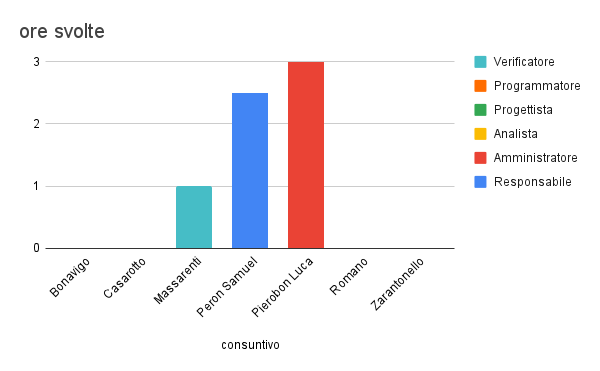
\includegraphics[width=12cm]{img/ore-usate.png}
\end{center}

\begin{table}[ht]
    \begin{tabularx}{\linewidth}{X|l|l}
    \rowcolor{gray!30}& Ore & Costo \\
    \hline
    
    Responsabile & 2,5 & € 70,00 \\
    \rowcolor{gray!10}Amministratore & 3 & € 60,00 \\
    Analista & 0 & € 0,00 \\
    \rowcolor{gray!10}Progettista & 0 & € 0,00 \\
    Programmatore & 0 & € 0,00 \\
    \rowcolor{gray!10}Verificatore & 1 &€ 15,00 \\
    totale & 6,5 & € 150,00 \\
    \end{tabularx}
    \caption{\label{costi-ruolo}Spartizione dei ruoli e ore svolte durante lo sprint}
\end{table}


Avendo quindi consumato €150,00\footnote{Si veda tabella \ref{costi-ruolo}} del budget durante questo sprint, rimangono ancora a disposizione € 13533,25 per gli sprint seguenti.

\subsection{Difficoltà e problemi di sprint}

Alcune questioni sono risultate durante questo sprint:

\begin{itemize}
    \item Alcune attività sono più lunghe dello sprint e non sono state spezzate abbastanza.
    \item Lo sprint potrebbe essere più lungo per evitare problemi di organizzazione. 
\end{itemize}

Queste verranno discusse in sede di preparazione del prossimo sprint.
